\chapter{Introduzione}
\section{tipologia in R}
\subsection{Distanza}
\begin{itemize}
\item {\color{red} $R$}: $d(x_1,x_2)=\abs{x_1-x_2}$
	\begin{figure}[ht]
		\centering
		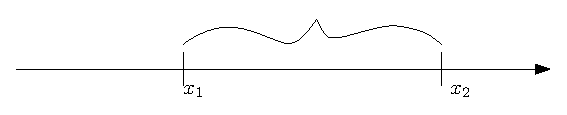
\includegraphics[width=6cm] {img/finiti/r.eps}
		\caption{distanza monodimensionale}
	\end{figure}
\item {\color{red} $R^2$}: Siano $P_1(x_1,y_1)$ e $P_2(x_2,y_2)$, la loro distanza è $d(P_1,P_2)=\sqrt{(x_2-x_1)^2+(y_2-y_1)^2}$
	\begin{figure}[ht]
		\centering
		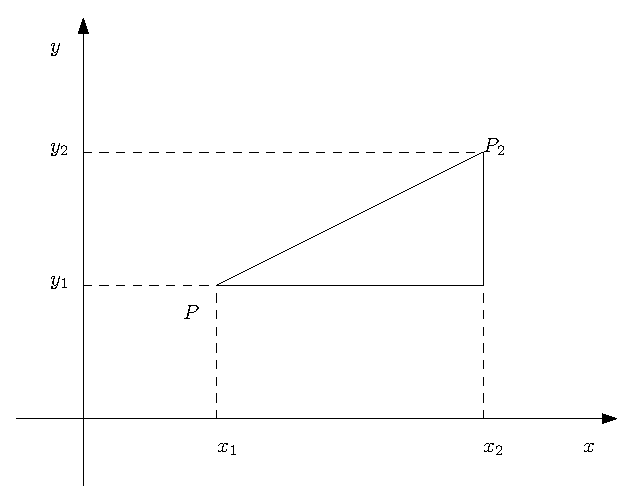
\includegraphics[width=4cm] {img/finiti/r2.eps}
		\caption{distanza bidimensionale}
	\end{figure}
\item {\color{red} $R^3$}: Siano $Q_1(x_2,y_2,z_2)$, la loro distanza è $d(Q_1,Q_2)=\sqrt{(x_2-x_1)^2+(y_2-y_1)^2+(z_2-z_1)^2}$
	\begin{figure}[ht]
		\centering
		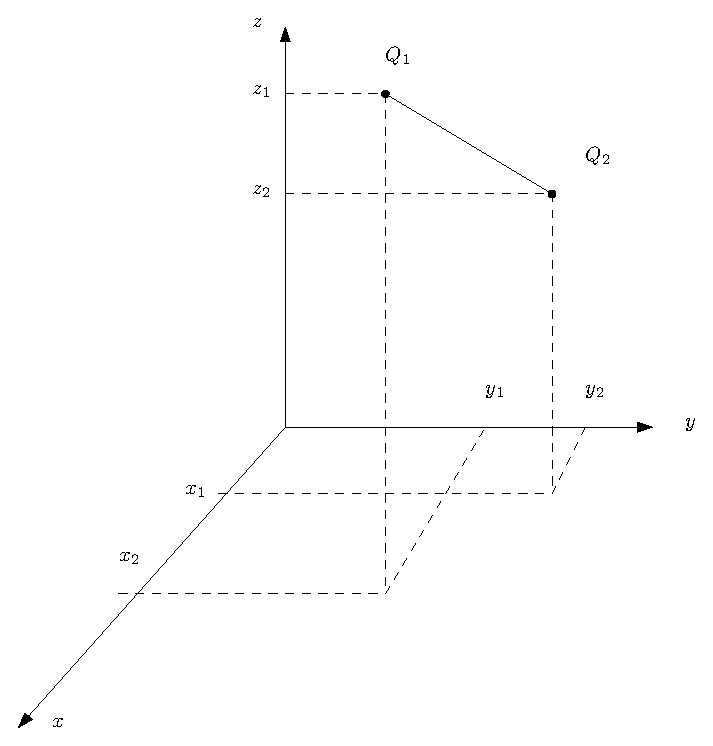
\includegraphics[width=4cm] {img/finiti/r3.eps}
		\caption{distanza tridimensionale}
	\end{figure}
\item {\color{red} $R^4$}: Siano $x=(x_1,x_2,x_3,\dots,x_n)\in R^n$ e $y=(y_1,y_2,y_3,\dots,y_n)\in R^n$
  \begin{equation*}
    d(x,y)=\sqrt{\sum^D_{a=1}(x_ay_a)^2}
  \end{equation*}
  La distanza è un'applicazione $R^n*R^n\to R^+\vee \{0\}$ (ha come immagine al più nullo)
\end{itemize}
\begin{pro}
  questi sono vincolati dalle sequenti proprietà
  \begin{itemize}
  \item $d(x,y)\leq 0$ $d(x,y)=0 \Leftrightarrow x\equiv y$ la distanza è nulla se i due punti coincidono
  \item $d(x,y) = d(y,x)$ la distanza tra $x$ e $y$ uguale alla distanza da $y$ a $x$
  \item $d(x,y)\geq d(x,y)+d(z,y)$ disuguaglianza triangolare.
  \end{itemize}
\end{pro}
\section{Intorno}
\begin{defi}
  Insieme dei punti che distano da un punto $P_0$ meno di un $\delta$
\end{defi}
\begin{itemize}
\item {\color{red} $R$} Intervallo $]x_0-\delta, x_0+\delta[$, P(x) generico punto $d(P_0,P)<\delta$
  \begin{equation*}
    \boxed{\abs{x-x_0}<\delta}
  \end{equation*}
\item {\color{red} $R^2$}
  \begin{equation*}
    \begin{matrix}
      P_0(x_0,y_0)\\
      P(x,y)\\
      d(P_0,P)<\delta\\
      \boxed{\sqrt{(x-x_0)^2+(y-y_0)^2}<\delta}
    \end{matrix}
  \end{equation*}
  Cerchio di cerntro $P_0$ e di perimetro $\delta$ privato della circonferenza.
\item {\color{red}$R^3$}
  \begin{equation*}
    \begin{matrix}
      Q_0(x_0,y_0,z_0) \\
      Q(x,y,z)\\
      d(Q,Q_0)<\delta\\
      \sqrt{(x-x_0)^2+(x-y_0)^2+(z-z_0)^2}<\delta
    \end{matrix}
  \end{equation*}
  Sfera di centro $Q_0$ e raggio $\delta$ privata della sua superficie.
\end{itemize}
\paragraph{Punto interno} $P_0$ è interno all'insieme D se:
\begin{equation}
    \exists I_{P_0,\delta} \subset D
\end{equation}
Esiste un interno di $P_0$ di ampiezza $\delta$ incluso nell'insieme $D$, cioè l'interno contiene tutti i
punti dell'insieme.
\paragraph{Punto esterno} $P_0$ è esterno all'insieme D se è interno al complementare di $D$, $CD$
\begin{equation}
    \exists I_{P_0,\delta}\subset CD
\end{equation}
esiste un interno di $P_0$ di ampiezza $\delta$ incluso nel complementare dell'interno D
\paragraph{Punto di frontiera} $P_0$ è un un punto di frontiera se
\begin{equation}
    P_0\in F_D \to \text{frontiera dell'insieme D}
\end{equation}
$\forall I_{F_D}$ in esso cadono punti di $D$ e punti di $CD$ qualunque interno, in esso cadono punti
dell'insieme $D$ e del suo complementare.
\paragraph{Punto di accumulazione}
$P_0$ è un punto di accumulazione se $\forall I_{P_0}$ cade in un punto $\in D$, se cade un punto di $D$
in $I_{p_0}$, allora ne cadono infiniti.
\paragraph{Punto isolato}
$P_0$ è un punto isolato se $\exists I_{P_0,\delta}$ in cui non cade nessun punto dell'insieme.
\paragraph{Insieme Aperto}
\begin{defi}
    $A$ si dice aperto se $\forall P \in A$ $\exists I_p \subset A$ per qualunque punto di A esiste un interno
    incluso in $A$, cioè ogni intorno di P è formato da punti dell'insieme aperto è formato da punti interni
    $]a:b[;\text{ } x^2+y^2<r^2$ cerchio senza circonferenza:
    \begin{equation}
        \begin{cases}
            y<1-x\\
            y>0 & \text{triangolo senza lati}\\
            0<x<1
        \end{cases}
    \end{equation}
\end{defi}
\subsection{Insieme chiuso}
\begin{defi}
  $A$ si dice chiuso se coincide con il suo insieme chiusura, che è formato dall'insieme stesso più gli
  eventuali punti di accumunlazione che non gli appartengono. Un insieme è chiuso quando contiene i suoi punti
  di accumulazione. $[a:b]; x^2+y^2\leq r^2$ cerchio più circonferenza:
  \begin{equation}
    \begin{cases}
        y\leq 1-x\\
        y\geq 0& \text{tringolo con lati}\\
        0\leq x\leq 1
    \end{cases} 
  \end{equation}
\end{defi}
\subsection{Insieme connesso}
\begin{defi}
  un insieme $A$ si dice connesso se e solo se $\forall P_1,P_2\subset A \text{ }
  \exists \Gamma i(P_1,P_2)\subset A$. A è connesso se per qualunque $P_1,P_2$ di $A$ esiste una spezzata
  inclusa in in $A$\\
  $A$ si dice {\color{red} semplicemente connessa} se qualunque chiusa inclusa in $A$ è frontiera dell'insieme.
\end{defi}
\subsection{Insieme convesso}
\begin{defi}
  un insieme $A$ si dice convesso se per ogni coppia di $x,y\in A$ il segmento $\bar{xy}$ è contenuto in A
\end{defi}
\begin{multicols}{2}
  \paragraph{Insiemi Limitati}
  In $R:A$ è limitato se $\forall x \in A:x\leq M$
  \begin{equation*}
    [-1;1]\text{ limitato}
  \end{equation*}
  In $R^2: A$ è limitato se è contenuto in un intorno circolare dell'origine
  \begin{equation}
    \exists M>0: \sqrt{x^2+y^2\leq M}
  \end{equation}
  \paragraph{Insieme illimitato}
  In $R: [2;+\infty [$ illimitato
  \begin{equation}
    In R^2: illimitato \begin{cases}
                         x\geq 0\\
                         y\geq 0
                       \end{cases}
  \end{equation}                     
\end{multicols}
\subsection{Coordinate Polari}
\begin{defi}
  in molti casi è utile utilizzare una funzione in coordinate polari, sia $P(x,y)$ un punto nel piano; esso
  è individuato univocamente da una coppia di valori: le coordinate cartesiano $X$ e $y$ oppure le coordinate
  polari $\rho$ e $\theta$.
  \begin{equation*}
    \begin{cases}
      \rho =\sqrt{x^2+y^2}\\
      x=\rho\cos\theta\\
      y=\rho\sin\theta
    \end{cases}
  \end{equation*}
  per capire, facciamo un esempio
  \begin{equation}
    f(x,y)=\frac{x^3}{x^2+y^2}\equiv f(\rho,\theta)=e^3\frac{\cos^2\theta}{e^2}
  \end{equation} 
\end{defi}
\subsection{Limiti e continuità}
\begin{defi}
  $f(x,y)$ una funzione definito in D e siano ($x_0,y_0$) punto di accumulazione per $D$
  \begin{equation}
    \begin{matrix}
      \lim\limits_{(x,y)\to(x_0,y_0)} f(x,y) = l & \forall\xi>0\text{ } \exists \delta_{(E)}>0:\forall I_{(x_0,y_0),\delta}
                                            /\{(x_0,y_0)\}, \forall(x,y)\in I | f(x,y)
    \end{matrix}
  \end{equation}
  Per qualunque $\xi > 0$ esiste un $\delta(\xi)>0$ per cui qualunque intorno di ($x_0,y_0$) al più $x_0,y_0$ e
  per qualunque $(x_0,y_0)$ di quest'intorno la funzione dista da i meno di $\xi$.
\end{defi}
\subsection{Continuità}
\begin{defi}
  Sia $f(x,y)$ definita in $D$, $f(x,y)$ si definisce {\color{red} continuo} in $(x_0,y_0)\in D$
  \begin{equation}
    \lim\limits_{(x,y)\to(x_0,y_0)}f(x,y)=f(x_0,y_0)
  \end{equation}
\end{defi}
\subsection{Esistenza del limite}
\begin{defi}
  Calcolando il limite con $f$ in forma polare esiste se non dipende da $\theta$. È possibile calcolare il
  limite di $f$ in forma cartesiano nel segmento nodo. Anziché considerare tutti i punti dell'interno, si
  considerino quelli su una generica retta.
  \begin{equation}
    y=y_0+m(x-x_0)
  \end{equation}
  \begin{itemize}
    \item Se il limite dipende da $m$ esso {\color{red} non esiste}.
    \item Se non dipende da $m$ {\color{red}esiste}.
  \end{itemize}  
\end{defi}
\subsection{Teorema di esistenza dei valori intermedi}
\begin{teorema}
  Sia $f(x,y)$ definita in un insieme chiuso e limitato. Allora $f(x,y)$ assume tutti i valori campresi fra
  il massimo ed il minimo di $f(x,y)$ su $D$
\end{teorema}
\subsection{Teorema di Weierstrass}
\begin{teorema}
  Una funzione continua in un intervallo chiuso e limitato, che ammette massimo e minimo assoluto.\\
  Sia $f(x,y)$ una funzione continua in D e sia D un insieme chiuso e limitato. Allora $f(x,y)$ ha
  massimo e minimo assoluto in D.
\end{teorema}
